% 03-familymask.tex — FamilyMask 染色体

\section{FamilyMask 多族 CA 编码}
\label{sec:familymask}

\subsection{设计动机}

经典 B/S 字符串把 8 邻域下活细胞和死细胞的 ``保留 / 翻转'' 决策压缩成两个 9-bit 集合, 搜索空间 $2^{18}$. 这个空间太小, 涌现复杂走廊结构 (1-cell 宽、长程连通、适度分叉) 的概率极低。Rejbrand 2017 年的网页笔记 \cite{rejbrand2017} 通过堆叠多个 B/S 字符串 + 优先级机制来扩展空间, 但缺乏形式化的染色体描述。

FamilyMask 把这种 ``多 B/S 字符串 + 优先级'' 的想法形式化为一条染色体: 最多 16 族并行, 每族独立持有邻域 mask、出生集、存活集与优先级; CA 每步按优先级遍历 active 族, 首个匹配的族决定下一态。这套结构把搜索空间从 $2^{18}$ 跃升至 $2^{1648}$ (16 slot $\times$ 103 bits/slot), 同时保留单族 B/S 字符串作为退化情形。

\subsection{染色体结构}

每条染色体由 16 个 \textbf{槽 (slot)} 组成, 每个槽对应一族规则 $\mathcal{F}_i = (\text{cells}_i, \text{birth}_i, \text{survive}_i, \text{priority}_i)$, 槽内数据布局为:
\begin{itemize}[leftmargin=*, itemsep=0pt, topsep=0pt]
  \item \textbf{active} (1 bit): 1 = 启用该族, 0 = 禁用。
  \item \textbf{cells} (80 bits): 邻域 mask, 标记 $9 \times 9$ 中心外 80 格中的 ``参与决策'' 格点 (1 = 计入, 0 = 忽略)。
  \item \textbf{birth} (9 bits): 死细胞在邻域中 ``活邻居数 $\in$ birth 集合'' 时复活。9 位对应 8 邻域下活邻居数 $0 \sim 8$ 加上 ``中心也计入'' 的 1 位扩展 (兼容 ``8 邻域 + 中心'' 与 ``纯 8 邻域'' 两种约定)。
  \item \textbf{survive} (9 bits): 同上, 但用于活细胞的存活判定。
  \item \textbf{priority} (4 bits): 0--15 的优先级, 数值小者先匹配。
\end{itemize}

每槽固定 103 bits ($= 1 + 80 + 9 + 9 + 4$); 16 槽共 1648 bits。

\begin{figure}[H]
\centering
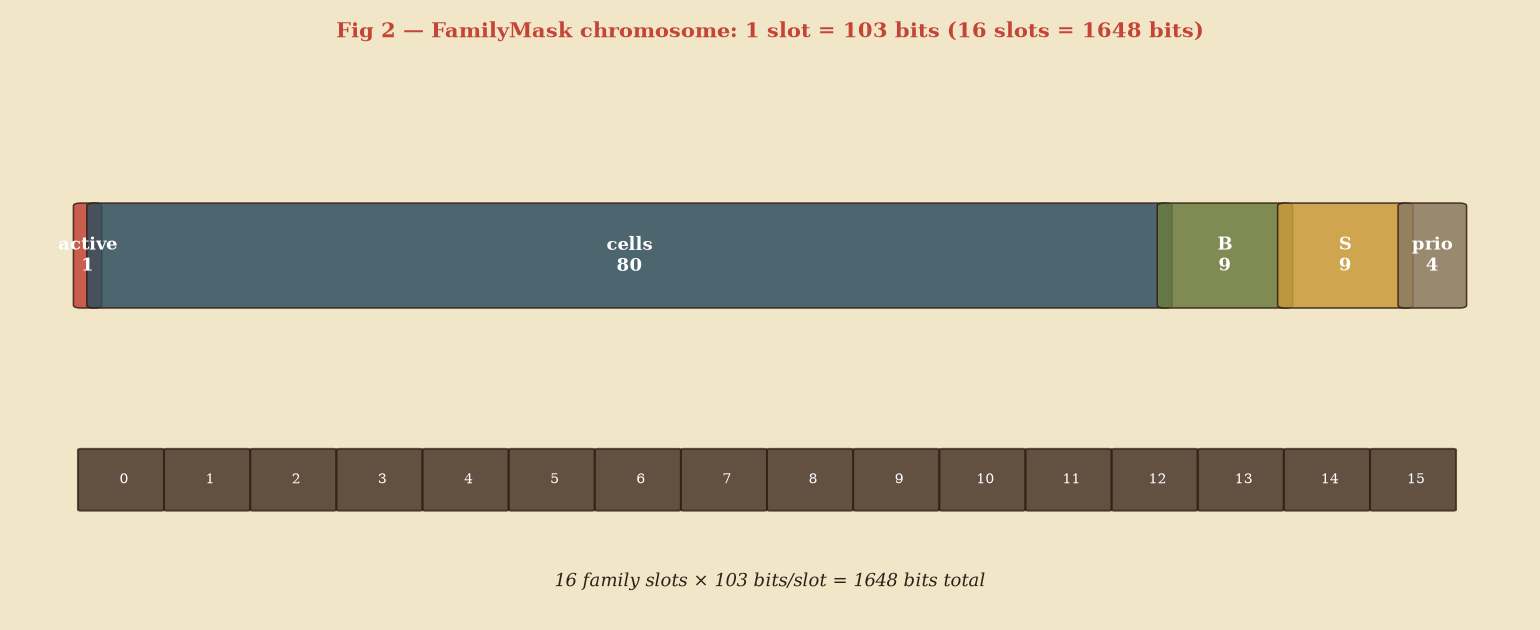
\includegraphics[width=0.95\linewidth]{../figures/v2/fig_chromosome_v3.png}
\caption{\textbf{FamilyMask 染色体结构示意 (以 8 族 / 16 槽为例)。}\\
上方两行共 16 个 \texttt{slot},F2/F5/F9/F12 (暖朱红填充) 示意 \texttt{active=1},
其余空白为 \texttt{active=0}。
每个 slot 内部 5 段分别为 \texttt{active} / cells mask (80 位) / B (9 位) / S (9 位) / priority (4 位), 共 103 位;
16 slot 共 1648 位。}
\label{fig:chrom}
\end{figure}

\subsection{执行语义}

记网格 $G \in \{0,1\}^{W \times H}$, $A \subseteq \{0, 1, \ldots, 15\}$ 为 active 族集合, $\text{cells}_i$ 为族 $i$ 的邻域 mask 集合 (80 个偏移量), $\text{birth}_i$ 与 $\text{survive}_i$ 分别为 $0 \sim 8$ 的子集加上 ``中心计入'' 位。CA 步 $t \to t+1$ 的更新规则:
\begin{align}
  n_i(x, y) &= \sum_{(\Delta x, \Delta y) \in \text{cells}_i} \mathbb{1}[G_t(x + \Delta x, y + \Delta y) > 0] \label{eq:ni}\\
  i^* &= \min\bigl\{\,i \in A : (G_t(x,y) = 0 \wedge n_i(x,y) \in \text{birth}_i) \vee (G_t(x,y) > 0 \wedge n_i(x,y) \in \text{survive}_i)\,\bigr\} \label{eq:istar}\\
  G_{t+1}(x, y) &=
  \begin{cases}
    1, & G_t(x, y) = 0 \wedge n_{i^*}(x, y) \in \text{birth}_{i^*} \\
    1, & G_t(x, y) > 0 \wedge n_{i^*}(x, y) \in \text{survive}_{i^*} \\
    0, & \text{otherwise}
  \end{cases} \label{eq:update}
\end{align}

若 $i^*$ 不存在 (即没有 active 族匹配), 元胞 $(x, y)$ 退化为 $\texttt{defaultState} = 0$ (墙)。

\subsection{搜索空间}

单族情形 ($|A| = 1$): 仅 cells mask 的 80 bits 与 B / S 的 9 bits 决定行为, 共 $2^{98}$ 有效组合 (priority 与 ``active'' 不参与决策); 若进一步约束 cells mask 为 ``8 邻域 (去掉中心)'', 退化为 $2^{18}$ 标准 B/S 字符串。

多族情形 ($|A| = k$): 每族独立贡献 $2^{103}$ 搜索空间, 全染色体 $2^{1648}$。但 ``早期匹配'' 语义 ($i^* = \min\{\ldots\}$) 使各族实际不独立, 优先级高的族会 ``截断'' 优先级低的族。

实际可遍历空间介于两者之间: ES 在 $2^{1648}$ 的 ``搜索空间大小'' 上做随机游走, 但因 ``早期匹配'' 截断, 有效搜索路径远小于 $2^{1648}$。这与神经架构搜索 (NAS) 中的情况类似: 更大的搜索空间不一定带来更好的均值, 但峰值通常更高 (本文 §6.1 在 (mask, maxFam) 消融中复现了这一点)。

\subsection{实现}

FamilyMask 在浏览器内通过 WebGPU compute shader 加速 CA 评估。每个 cell 的 update (\ref{eq:ni})--(\ref{eq:update}) 在 WGSL kernel 中并行执行, dispatch 维度 $(\text{ruleCount} \times \text{seedCount}, \text{cellCount})$。ES 评估的耗时瓶颈在 $n_i$ 的邻域求和, 80 cells mask 在 $40 \times 60$ 网格上单步需要 $\sim$ 0.1 ms (WebGPU, 主流 GPU)。
